\section{Iteración 4}
\label{sec:iteracion_4}

% Al igual que al principio de la segunda iteración, se esperan los resultados de las pruebas realizadas para poder empezar con la planificación de la tercera iteración.
%
% \subsection{Iteration Planning Meeting}
% \label{sub:iteration2_planning_meeting}
%
%
% Los resultados de las pruebas realizadas se analizan para determinar si los criterios de aceptación, de las historias de usuario trabajadas en la segunda iteración, se cumplen para poder continuar con las historias que continúan sin ser desarrolladas, en caso que las pruebas fallen, es necesario continuar con la implementación de las historias inconclusas.\\
%
% En el caso del presente proyecto, las pruebas pasaron exitosamente y se aceptaron los criterios de aceptación de las historias de usuario trabajadas, por lo tanto se procede con la primera fase del “Iteration Planning”. \\
%

\subsection{Planificación de la Iteración 4}

% Esta fase generalmente se realiza en 2 pasos pero será realizada al mismo tiempo, ya que en la exploración se definen las tareas a realizar y en la planeación se asigna estas tareas al equipo de desarrollo, el cual tiene que estimar las tareas, pero como el equipo de desarrollo está compuesto por mi persona, puedo definir las tareas y asignarles una estimación en el mismo paso.\\
%
% En la Iteración 4, se trabajaron las historias de usuario 5, 8 y 9. A continuacion se puede ver las tareas de ingenieria con su respectiva estimacion para las historias de usuario ya mencionadas.


% \subsubsection{Tareas del US05}
% \label{sub:us05_tasks}

A continuación se analizará la \emph{historia de usuario} US05, ver el cuadro \ref{tab:US05}.

  
\begin{table}[H]
\begin{center}
\begin{tabularx}{0.75\textwidth}{ X }
  \toprule
  \textbf{Historia de Usuario:} US05
  \makebox[6cm][r]{\textbf{Prioridad:} Alta} \\
  \makebox[4cm][r]{}
  \makebox[6cm][r]{\textbf{Riesgo:} Alto} \\

  \addlinespace
  \textbf{Nombre:} Implementar el modulo de Registro de un Visitante.\\

  \addlinespace
  \textbf{Descripción:} \\
  \tab Yo como visitante.\\
  \tab Deseo registrarme. \\
  \tab Para tener mas opciones dentro el sistema. \\

  \addlinespace
  \textbf{Criterios de Aceptación:} \\
  \tab Quiero ver un formulario donde me pueda registrar. \\
  \tab Una vez registrado quiero poder ingresar al sistema con mis credenciales. \\
  \tab Quiero ver tener la posibilidad de editar mis datos. \\

  \bottomrule
\end{tabularx}
\caption{Historia de Usuario - US05}
\label{tab:US05}
\end{center}
\end{table}


  \begin{table}[H]
  \begin{center}
    \begin{tabularx}{0.75\textwidth}{ X }
      \toprule
      \textbf{Número de Tarea:} T028
      \makebox[1cm][r]{}
      \makebox[6cm][r]{\textbf{Historia de Usuario:} US05} \\

      \addlinespace
      \textbf{Descripción:} Generar un link para acceder al formulario de registro. \\

      \addlinespace
      \textbf{Tipo de Tarea:} Desarrollo
      \makebox[6cm][r]{\textbf{Estimación [dias]:} 0.5} \\

      \addlinespace
      \textbf{Programador Responsable:} Edmundo Figueroa \\

      \bottomrule
    \end{tabularx}
    \caption{Tarea de Ingeniería - T028}
    \label{tab:T028}
  \end{center}
\end{table}


\begin{table}[H]
  \begin{center}
    \begin{tabularx}{0.75\textwidth}{ X }
      \toprule
      \textbf{Número de Tarea:} T029
      \makebox[1cm][r]{}
      \makebox[6cm][r]{\textbf{Historia de Usuario:} US05} \\

      \addlinespace
      \textbf{Descripción:} Mostrar un formulario con el nombre, el email y la razon para registrarse. \\

      \addlinespace
      \textbf{Tipo de Tarea:} Desarrollo
      % \makebox[1cm][r]{}
      \makebox[6cm][r]{\textbf{Estimación [dias]:} 0.5} \\

      \addlinespace
      \textbf{Programador Responsable:} Edmundo Figueroa \\

      \bottomrule
    \end{tabularx}
    \caption{Tarea de Ingeniería - T029}
    \label{tab:T029}
  \end{center}
\end{table}

\begin{table}[H]
  \begin{center}
    \begin{tabularx}{0.75\textwidth}{ X }
      \toprule
      \textbf{Número de Tarea:} T030
      \makebox[1cm][r]{}
      \makebox[6cm][r]{\textbf{Historia de Usuario:} US05} \\

      \addlinespace
      \textbf{Descripción:} Implementar un modulo de Registro de Usuarios. \\

      \addlinespace
      \textbf{Tipo de Tarea:} Desarrollo
      \makebox[6cm][r]{\textbf{Estimación [dias]:} 2} \\

      \addlinespace
      \textbf{Programador Responsable:} Edmundo Figueroa \\

      \bottomrule
    \end{tabularx}
    \caption{Tarea de Ingeniería - T030}
    \label{tab:T030}
  \end{center}
\end{table}


% \subsubsection{Tareas del US08}
% \label{sub:us08_tasks}

A continuación se analizará la \emph{historia de usuario} US08, ver el cuadro \ref{tab:US08}.

  
\begin{table}[H]
\begin{center}
\begin{tabularx}{0.75\textwidth}{ X }
 \toprule
 \textbf{Historia de Usuario:} US08
 \makebox[6cm][r]{\textbf{Prioridad:} Alta} \\
 \makebox[4cm][r]{}
 \makebox[6cm][r]{\textbf{Riesgo:} Alto} \\

 \addlinespace
 \textbf{Nombre:} Implementar el módulo para Administrar Usuarios.\\

 \addlinespace
 \textbf{Descripción:} \\
 \tab Yo como usuario administrador.\\
 \tab Deseo administrar usuarios. \\
 \tab Para añadir o remover usuarios del sistema. \\

 \addlinespace
 \textbf{Criterios de Aceptación:} \\
 \tab Quiero ver los usuarios que desean registrarse en el sistema. \\
 \tab Quiero aceptar o rechazar solicitudes de registro. \\
 \tab Quiero eliminar usuarios que no usen el sistema de forma adecuada. \\

 \bottomrule
\end{tabularx}
\caption{Historia de Usuario - US08}
\label{tab:US08}
\end{center}
\end{table}


  \begin{table}[H]
  \begin{center}
    \begin{tabularx}{0.75\textwidth}{ X }
      \toprule
      \textbf{Número de Tarea:} T031
      \makebox[1cm][r]{}
      \makebox[6cm][r]{\textbf{Historia de Usuario:} US08} \\

      \addlinespace
      \textbf{Descripción:} Mostrar el Menú de Registros solo para usuario Administrador. \\

      \addlinespace
      \textbf{Tipo de Tarea:} Desarrollo
      \makebox[6cm][r]{\textbf{Estimación [dias]:} 0.5} \\

      \addlinespace
      \textbf{Programador Responsable:} Edmundo Figueroa \\

      \bottomrule
    \end{tabularx}
    \caption{Tarea de Ingeniería - T031}
    \label{tab:T031}
  \end{center}
\end{table}


\begin{table}[H]
  \begin{center}
    \begin{tabularx}{0.75\textwidth}{ X }
      \toprule
      \textbf{Número de Tarea:} T032
      \makebox[1cm][r]{}
      \makebox[6cm][r]{\textbf{Historia de Usuario:} US08} \\

      \addlinespace
      \textbf{Descripción:} Mostrar una lista con los Usuarios a registrar. \\

      \addlinespace
      \textbf{Tipo de Tarea:} Desarrollo
      % \makebox[1cm][r]{}
      \makebox[6cm][r]{\textbf{Estimación [dias]:} 1} \\

      \addlinespace
      \textbf{Programador Responsable:} Edmundo Figueroa \\

      \bottomrule
    \end{tabularx}
    \caption{Tarea de Ingeniería - T032}
    \label{tab:T032}
  \end{center}
\end{table}

\begin{table}[H]
  \begin{center}
    \begin{tabularx}{0.75\textwidth}{ X }
      \toprule
      \textbf{Número de Tarea:} T033
      \makebox[1cm][r]{}
      \makebox[6cm][r]{\textbf{Historia de Usuario:} US08} \\

      \addlinespace
      \textbf{Descripción:} Mostrar un botón para aceptar del registro del usuario. \\

      \addlinespace
      \textbf{Tipo de Tarea:} Desarrollo
      \makebox[6cm][r]{\textbf{Estimación [dias]:} 0.5} \\

      \addlinespace
      \textbf{Programador Responsable:} Edmundo Figueroa \\

      \bottomrule
    \end{tabularx}
    \caption{Tarea de Ingeniería - T033}
    \label{tab:T033}
  \end{center}
\end{table}

\begin{table}[H]
  \begin{center}
    \begin{tabularx}{0.75\textwidth}{ X }
      \toprule
      \textbf{Número de Tarea:} T034
      \makebox[1cm][r]{}
      \makebox[6cm][r]{\textbf{Historia de Usuario:} US08} \\

      \addlinespace
      \textbf{Descripción:} Mostrar un botón para Rechazar del registro del usuario. \\

      \addlinespace
      \textbf{Tipo de Tarea:} Desarrollo
      \makebox[6cm][r]{\textbf{Estimación [dias]:} 0.5} \\

      \addlinespace
      \textbf{Programador Responsable:} Edmundo Figueroa \\

      \bottomrule
    \end{tabularx}
    \caption{Tarea de Ingeniería - T034}
    \label{tab:T034}
  \end{center}
\end{table}

\begin{table}[H]
  \begin{center}
    \begin{tabularx}{0.75\textwidth}{ X }
      \toprule
      \textbf{Número de Tarea:} T035
      \makebox[1cm][r]{}
      \makebox[6cm][r]{\textbf{Historia de Usuario:} US08} \\

      \addlinespace
      \textbf{Descripción:} Mostrar una lista con Usuarios Registrados. \\

      \addlinespace
      \textbf{Tipo de Tarea:} Desarrollo
      \makebox[6cm][r]{\textbf{Estimación [dias]:} 0.5} \\

      \addlinespace
      \textbf{Programador Responsable:} Edmundo Figueroa \\

      \bottomrule
    \end{tabularx}
    \caption{Tarea de Ingeniería - T035}
    \label{tab:T035}
  \end{center}
\end{table}

\begin{table}[H]
  \begin{center}
    \begin{tabularx}{0.75\textwidth}{ X }
      \toprule
      \textbf{Número de Tarea:} T036
      \makebox[1cm][r]{}
      \makebox[6cm][r]{\textbf{Historia de Usuario:} US08} \\

      \addlinespace
      \textbf{Descripción:} Implementar un botón para eliminar Usuarios. \\

      \addlinespace
      \textbf{Tipo de Tarea:} Desarrollo
      \makebox[6cm][r]{\textbf{Estimación [dias]:} 0.5} \\

      \addlinespace
      \textbf{Programador Responsable:} Edmundo Figueroa \\

      \bottomrule
    \end{tabularx}
    \caption{Tarea de Ingeniería - T036}
    \label{tab:T036}
  \end{center}
\end{table}


  % \subsubsection{Tareas del US09}
  % \label{sub:us09_tasks}

  A continuación se analizará la \emph{historia de usuario} US09, ver el cuadro \ref{tab:US09}.

    
\begin{table}[H]
\begin{center}
\begin{tabularx}{0.75\textwidth}{ X }
\toprule
\textbf{Historia de Usuario:} US09
\makebox[6cm][r]{\textbf{Prioridad:} Alta} \\
\makebox[4cm][r]{}
\makebox[6cm][r]{\textbf{Riesgo:} Alto} \\

\addlinespace
\textbf{Nombre:} Implementar el reporte de los lugares más visitados.\\

\addlinespace
\textbf{Descripción:} \\
\tab Yo como usuario administrador.\\
\tab Deseo ver los lugares más visitados. \\
\tab Para obtener información y estadísticas de los lugares dentro del campus Universitario. \\

\addlinespace
\textbf{Criterios de Aceptación:} \\
\tab Quiero ver la cantidad de veces que los usuarios buscan un lugar. \\
\tab Quiero poder guardar el reporte. \\

\bottomrule
\end{tabularx}
\caption{Historia de Usuario - US09}
\label{tab:US09}
\end{center}
\end{table}


    \begin{table}[H]
  \begin{center}
    \begin{tabularx}{0.75\textwidth}{ X }
      \toprule
      \textbf{Número de Tarea:} T037
      \makebox[1cm][r]{}
      \makebox[6cm][r]{\textbf{Historia de Usuario:} US09} \\

      \addlinespace
      \textbf{Descripción:} Implementar un módulo de Reportes. \\

      \addlinespace
      \textbf{Tipo de Tarea:} Desarrollo
      \makebox[6cm][r]{\textbf{Estimación [dias]:} 1} \\

      \addlinespace
      \textbf{Programador Responsable:} Edmundo Figueroa \\

      \bottomrule
    \end{tabularx}
    \caption{Tarea de Ingeniería - T037}
    \label{tab:T037}
  \end{center}
\end{table}


\begin{table}[H]
  \begin{center}
    \begin{tabularx}{0.75\textwidth}{ X }
      \toprule
      \textbf{Número de Tarea:} T038
      \makebox[1cm][r]{}
      \makebox[6cm][r]{\textbf{Historia de Usuario:} US09} \\

      \addlinespace
      \textbf{Descripción:} Mostrar el menú de Reportes. \\

      \addlinespace
      \textbf{Tipo de Tarea:} Desarrollo
      % \makebox[1cm][r]{}
      \makebox[6cm][r]{\textbf{Estimación [dias]:} 0.5} \\

      \addlinespace
      \textbf{Programador Responsable:} Edmundo Figueroa \\

      \bottomrule
    \end{tabularx}
    \caption{Tarea de Ingeniería - T038}
    \label{tab:T038}
  \end{center}
\end{table}

\begin{table}[H]
  \begin{center}
    \begin{tabularx}{0.75\textwidth}{ X }
      \toprule
      \textbf{Número de Tarea:} T039
      \makebox[1cm][r]{}
      \makebox[6cm][r]{\textbf{Historia de Usuario:} US09} \\

      \addlinespace
      \textbf{Descripción:} Mostrar el Reporte de Frecuencia. \\

      \addlinespace
      \textbf{Tipo de Tarea:} Desarrollo
      \makebox[6cm][r]{\textbf{Estimación [dias]:} 0.5} \\

      \addlinespace
      \textbf{Programador Responsable:} Edmundo Figueroa \\

      \bottomrule
    \end{tabularx}
    \caption{Tarea de Ingeniería - T039}
    \label{tab:T039}
  \end{center}
\end{table}

\begin{table}[H]
  \begin{center}
    \begin{tabularx}{0.75\textwidth}{ X }
      \toprule
      \textbf{Número de Tarea:} T040
      \makebox[1cm][r]{}
      \makebox[6cm][r]{\textbf{Historia de Usuario:} US09} \\

      \addlinespace
      \textbf{Descripción:} Mostrar un botón para Guardar el Reporte generado. \\

      \addlinespace
      \textbf{Tipo de Tarea:} Desarrollo
      \makebox[6cm][r]{\textbf{Estimación [dias]:} 0.5} \\

      \addlinespace
      \textbf{Programador Responsable:} Edmundo Figueroa \\

      \bottomrule
    \end{tabularx}
    \caption{Tarea de Ingeniería - T040}
    \label{tab:T040}
  \end{center}
\end{table}



    \subsection{Implementación de la Iteración 4}


        \subsubsection{Registro de Usuarios}

El registro de Usuarios sera mediante un formulario con el nombre, el email y la razon del registrante, y solamente el usuario administrador sera capaz de aceptar o rechazar la solicitud de registro, para lo cual se implemento en la aplicacion el \emph{formulario de registro} y el menu de \emph{menu de registros}. \\



\begin{description}
  \item[Formulario de Registro:] Para completar esta tarea se implemento en la vista de la aplicacion el formulario, ver la figura \ref{fig:registro_form} usando \emph{ember-paper}, que como ya se menciono es la libreria usada para implementar la vista de la aplicacion dandole el ``look and feel'' de una aplicacion movil. \\

  \begin{figure}[H]
        \begin{center}
          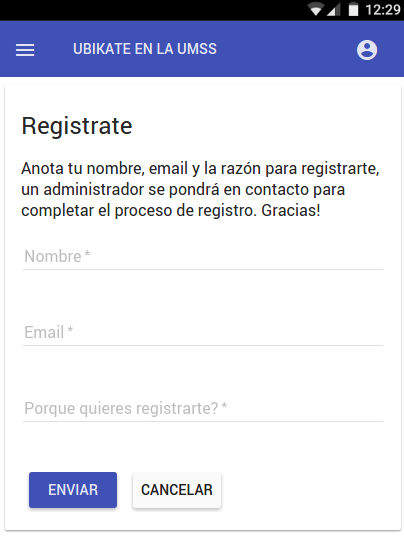
\includegraphics[width=0.5\textwidth]{registro_form}

          \caption{Formulario para Registro de Usuario}
          \label{fig:registro_form}
          \caption*{Fuente: Elaboración propia.}
        \end{center}
  \end{figure}


  Posteriormente se implemento en el \emph{backend} de la aplicacion el modulo para guardar la solicitud de registro, para lo cual se  anadio el \emph{endpoint} en el API que escuche la peticion POST generada al aceptar el \emph{formulario de registro}, este \emph{endpoint} inserta los datos colectados por el navegador en la base de datos para que esten disponibles posteriormente en el \emph{Menu de Registros}.\\


  \item[Menu de Registros] El \emph{menu de registro} sera donde un usuario administrador puede ver todas las solicitudes de registro, y de acuerdo de la \emph{razon} de registro se puede determinar si la solicitud es de parte de un usuario responsable, en caso de necesitar mas informacion del registrante se puede usar el \emph{email} enviado, una ves que el administrador considera que el registrante no va a jugar en el sistema para asegurar la integridad de la misma, puede \emph{aceptar} el registro, de esta forma el usuario recibira un email donde se confirma el registro al sistema.\\





\end{description}


\subsubsection{Generacion del Reporte}

Para la implementacion del modulo que genere un reporte, se tuvo que modificar la tabla de los lugares, para saber cuantas veces un ``lugar'' es buscado, con esta informacion se puede proporcionar un reporte de frecuencia, para tal efecto se uso \emph{ember-charts}, que como se puede observar en el codigo \ref{chart_template}, solo se necesita una linea para crear el reporte de frecuencia de la figura \ref{fig:reporte} \\

\begin{center}
  \begin{lstlisting}[label=chart_template,caption=Componente de \emph{Ember-charts}.]

{{horizontal-bar-chart data=model selectedSeedColor="green" sortAscending=false}}

  \end{lstlisting}
\end{center}

\begin{figure}[H]
      \begin{center}
        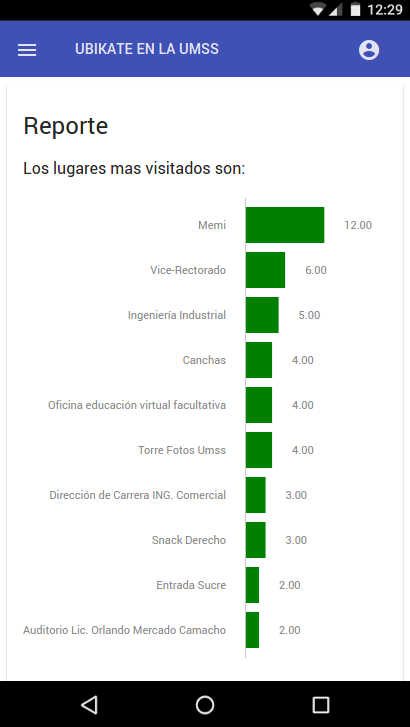
\includegraphics[width=0.5\textwidth]{reporte}

        \caption{Reporte de Frecuencia}
        \label{fig:reporte}
        \caption*{Fuente: Elaboración propia.}
      \end{center}
\end{figure}



Este reporte es obtiene al conocer la cantidad de veces que los usuarios han buscado un ``lugar'' mediante el SQL query, que se puede ver en el codigo \ref , el cual discrimina los primeros 10 lugares mas buscados dentro del campus universitario, ya que al existir tantas aulas y oficinas el reporte se haria muy extenso. \\

\begin{center}
  \begin{lstlisting}[label=request_visited,caption=Insertar un ``lugar'' en la base de datos.]

    router.get('places/visited/count',  (req, res) => {
      Place.forge()
        .where('visit_count', '>', '1')
        .orderBy('visit_count', 'DESC')
        .query((qb) => qb.limit(10))
        .fetchAll({columns: ["name as label", "visit_count as value"]})
        .then((visited) => {
            res.json(visited.toJSON());
        })
        .catch((err) => {
            res.status(500);
        });
    });

  \end{lstlisting}
\end{center}

%
%     \subsection{Registrar el Avance}
%     \label{sub:iteracion4_avance}

  \subsection{Pruebas de Aceptación de la Iteración 4}


    \begin{table}[H]
  \begin{center}
    \begin{tabularx}{0.75\textwidth}{ X }
      \toprule
      \textbf{Codigo:} CP008
      \makebox[3cm][r]{}
      \makebox[6cm][r]{\textbf{Historia de Usuario:} US005} \\

      \addlinespace
      \textbf{Nombre:} Verificar el Formulario de Registro \\

      \addlinespace
      \textbf{Descripción:} Validar que un usuario puede ver el formulario de registro. \\

      \addlinespace
      \textbf{Condiciones de Ejecución:} El usuario no está registrado. \\

      \addlinespace
      \textbf{Entradas / Pasos de Ejecución:}  \\
      \tab \textbf{1.} Seleccionar el link \emph{Registrarse}. \\
      \tab \textbf{2.} Ingresar el Nombre del usuario.\\
      \tab \textbf{3.} Ingresar el Email del usuario.\\
      \tab \textbf{4.} Ingresar una Razón de registro.\\
      \tab \textbf{5.} Aceptar el envío del formulario.\\


      \addlinespace
      \textbf{Resultado Esperado:} El Usuario recibe un email de confirmación de Email.  \\

      \addlinespace
      \textbf{Evaluación de la Prueba:} Prueba exitosa. \\

      \bottomrule
    \end{tabularx}
    \caption{Caso de Prueba - CP008}
    \label{tab:CP008}
  \end{center}
\end{table}


\begin{table}[H]
  \begin{center}
    \begin{tabularx}{0.75\textwidth}{ X }
      \toprule
      \textbf{Codigo:} CP009
      \makebox[3cm][r]{}
      \makebox[6cm][r]{\textbf{Historia de Usuario:} US008} \\

      \addlinespace
      \textbf{Nombre:} Verificar el Registro del Usuario \\

      \addlinespace
      \textbf{Descripción:} La prueba verifica que un usuario se puede registrar en el sistema.\\

      \addlinespace
      \textbf{Condiciones de Ejecución:} El usuario ha ingresado datos válidos a la solicitud de registro.  \\

      \addlinespace
      \textbf{Entradas / Pasos de Ejecución:}  \\
      \tab \textbf{1.} El Administrador ingresa al \emph{Menú de Registros}. \\
      \tab \textbf{2.} Confirma la validez de los datos de registro del usuario.\\
      \tab \textbf{3.} Acepta el registro del usuario.\\

      \addlinespace
      \textbf{Resultado Esperado:} El usuario recibe un email de confirmación de registro. \\

      \addlinespace
      \textbf{Evaluación de la Prueba:} Prueba exitosa. \\

      \bottomrule
    \end{tabularx}
    \caption{Caso de Prueba - CP009}
    \label{tab:CP009}
  \end{center}
\end{table}

\begin{table}[H]
  \begin{center}
    \begin{tabularx}{0.75\textwidth}{ X }
      \toprule
      \textbf{Codigo:} CP010
      \makebox[3cm][r]{}
      \makebox[6cm][r]{\textbf{Historia de Usuario:} US009} \\

      \addlinespace
      \textbf{Nombre:} Verificar el Reporte de frecuencia. \\

      \addlinespace
      \textbf{Descripción:} La prueba verifica que el usuario puede ver el reporte de frecuencia.\\

      \addlinespace
      \textbf{Condiciones de Ejecución:} El usuario debe tener permisos de Administrador.  \\

      \addlinespace
      \textbf{Entradas / Pasos de Ejecución:}  \\
      \tab \textbf{1.} El usuario ingresa al sistema con permisos de Administrador. \\
      \tab \textbf{2.} Selecciona al menú de \emph{Reportes}. \\

      \addlinespace
      \textbf{Resultado Esperado:} El usuario puede ver la gráfica de barras con los lugares más visitados. \\

      \addlinespace
      \textbf{Evaluación de la Prueba:} Prueba exitosa. \\

      \bottomrule
    \end{tabularx}
    \caption{Caso de Prueba - CP010}
    \label{tab:CP010}
  \end{center}
\end{table}

